\chapter{眶额皮层:基于输出结果选择目的}
这本书提出了关于灵长类动物前额叶皮层基本功能的方案。

\section{概述}
眶额皮层有助于评估和选择对象未来行动的目标及其联系解释了其独特的功能。 它与嗅觉、内脏、味觉、体感和皮层的视觉区域,这些信号的结合产生了丰富的,特定结果的高维表示,一个由想象。 眶额皮层与杏仁核更新的相互作用根据当前的生物学需求评估这些成果。由于这些联系,看到有营养的食物或视觉标志与他们相关联唤起他们的味道和他们当前的动机价值。 虽然眶额皮层的很大一部分将物体链接到特定的结果,另一部分对一般结果这样做,在“共同货币”。 通过将行为结果分配给特定的觅食事件,而不是此类事件的平均值,眶额皮层灵长类动物提供了关键的选择优势。
\section{介绍}
第 3 章论证了内侧皮层的连接允许它做出选择在行动中,特别是当这些选择发生在没有外部感官的情况下时告诉动物该做什么的提示。 本章介绍眶额皮层。 它认为眶额皮层的连接允许它为外部提示做选择内侧皮层对“内部”提示的作用。\par
与内侧皮层一样,眶额皮层既有颗粒状部分,也有颗粒状部分。第 2 章论证了早期哺乳动物进化出的颗粒状部分,而颗粒状部分部分在早期灵长类动物中进化。 与第 3 章一样,我们需要利用老鼠的证据深入了解颗粒状的。 原因是一样的:我们对灵长类动物的无颗粒皮层。 也像第 3 章一样,我们需要说什么是粒度部分眶额皮层可以做到其颗粒部分不能做到的。 我们采纳这个想法灵长类动物的眼眶额皮层使用单个事件将特定结果与导致这些结果的选择:一种刺激-结果关联的形式。\par
显然,大多数动物都可以学习刺激-结果关联。巴甫洛夫条件反射依赖于它,就像仪器条件反射依赖于学习行动—结果关联一样。 除了无柄形式,我们假设所有动物物种都可以是仪器和经典条件。 所以我们面临一个挑战:我们需要说什么哺乳动物眶额皮层的颗粒部分以及颗粒部分是什么灵长类动物的眶 额皮层。\par
在本章中,我们区分了刺激-结果关联的两个方面。 首先涉及刺激和结果之间的预测关系:可能性给定刺激就会发生结果。 第二个涉及评估结果在当前生物学需求方面的价值。 这两个方面,我们分别称为关联映射和动机评估,都会影响觅食选择,并且两者需要随着情况的变化而更新。\par
\section{区域}
图 4.1 说明了人类和猴子的眶额皮层,图 2.1 说明了其细分的一个视图。 在猕猴中,第 11 区位于它的喙部,区域 13 和 14 位于更靠后的位置 (Walker 1940)。 在灵长类动物中,大部分皮质具有颗粒状细胞结构,但区域 13 和 14 的尾部是颗粒状的,邻近的前岛叶皮质也是如此。 继 Carmichael 和 Price(1994)之后,我们将所有这些无颗粒区域包括在眶额皮层中。 为了清楚起见,我们有时使用眶额皮层的缩写 OFC。 我们尤其在讨论时这样做OFC的分支机构。\par
我们将区域 12/47 的部分从此处解释的眶额皮层延伸到半球的轨道表面,以及极地皮层(区域 10)。
\begin{figure}[!htb]
	\centering
	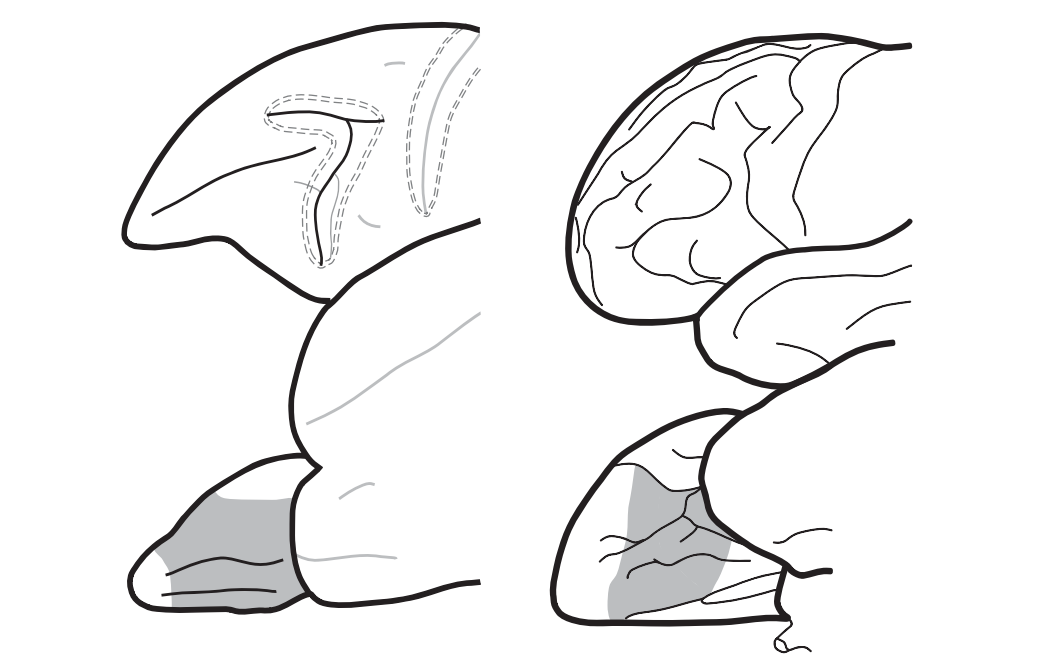
\includegraphics{image_pfc/Fig_4_1}
	\caption{猴子(左)和人类(右)的眶额皮层。 格式如图 1.2 所示。}
	\label{fig:fig}
\end{figure}


\section{连接}
图 4.2 说明了眶额皮层的选定连接,这表明以下结论:\par
1. 与杏仁核最密集的连接涉及眶额皮层的颗粒部分,优先与杏仁核的基底外侧核连接。然而,13 区的颗粒状部分也与杏仁核有关,其他粒度细分(见图 3.3)(Carmichael \& Price 1995a)。\par
\begin{figure}[!htb]
	\centering
	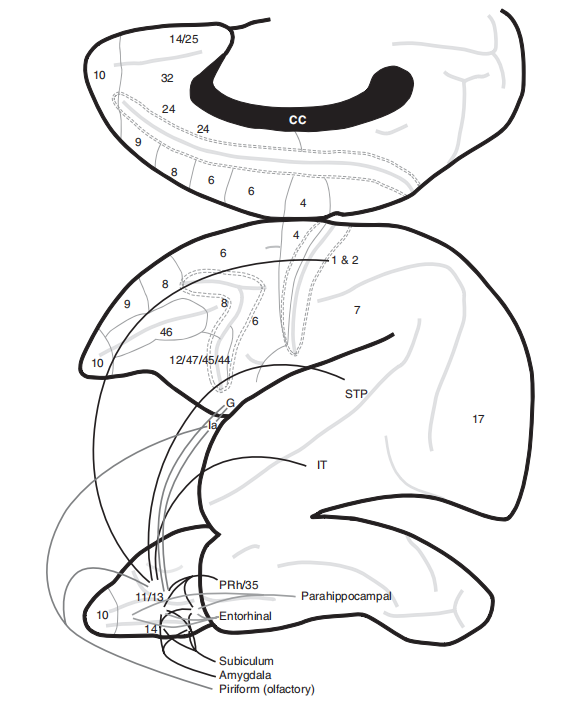
\includegraphics{image_pfc/Fig_4_2}
	\caption{眶额皮层的选定连接。 图 1.4 和 1.5 给出了脑沟和区域的名称。 线连接一些与轨道有直接轴突连接的区域,除非另有说明,否则假设是相连的。}
	\label{fig:fig}
\end{figure}
2. 无颗粒岛叶皮层接收来自味觉和梨状(嗅觉)皮层(Carmichael \& Price 1995a)。 它还接收来自脑干和丘脑的内脏信号 (Ray \& Price 1992)。 后者包括传达反映动物新陈代谢状态的信号的感觉,例如,缺氧或低血糖,以及来自肺、心脏、压力感受器和消化道 (Craig 2002)。 这些发现导致了这样一种观点,即颗粒状岛叶皮质在内感受中发挥作用。\par
3. 嗅觉、味觉和内脏信息从其到达颗粒状 OFC颗粒部分(Carmichael \& Price 1994)。该信息可以在颗粒皮层中与来自颞下皮层的视觉输入相结合,目标区域 13和 11,以及从投射到区域 13 的鼻周皮质(Saleem 等人,2008 年)。后一种投影提供了关于物体的多模态信息 (Murray et al.
2007 年)。
\subsection{损伤和激活}

\subsection{损伤和活动}

\subsection{活动和激活}




\subsection{结论}


